\section{Theory}
\subsection{Euler's Turbomachinery Equations}
\begin{figure}[h]
    \centering
    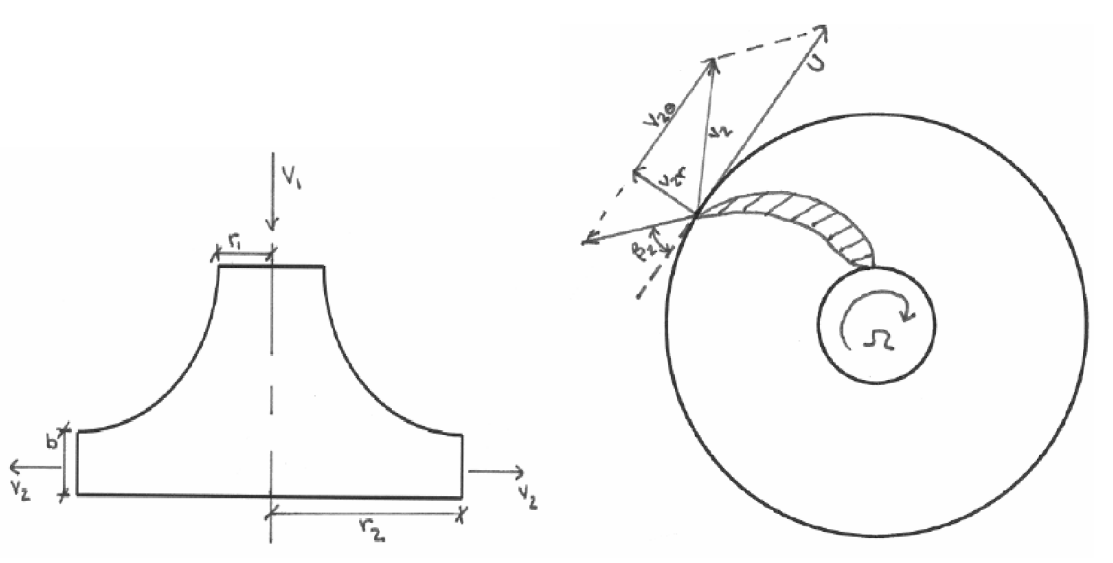
\includegraphics[width=0.5\textwidth]{Sections/Figures/theory impeller diagram.png}
    \caption{Impeller force and acceleration diagrams.}
    \label{fig:impeller}
\end{figure}
\noindent Using the following assumptions:
\begin{enumerate}
    \item Viscous effects are negligible
    \item Velocity profile is uniform at the exit
    \item All work done by the pump is transferred to the fluid
\end{enumerate}
Then by conservation of angular momentum,
\begin{align}
    T = \dot{m} r_2 v_{2\theta} \label{eq:torque}
\end{align}
where $T$ is the torque, $\dot{m}$ is the mass flow rate, $r_2$ is the radius of the impeller, and $v_{2\theta}$ is the tangential velocity at the exit. From Figure \ref{fig:impeller}, we can see that 
\begin{align}
    v_{2\theta} = U - v_{2r} \cot{\beta_2} \label{eq:vtheta}
\end{align}
where $U$ is the tip speed, $v_{2r}$ is the radial velocity at the exit, and $\beta_2$ is the blade angle. Combining (\ref{eq:torque}) and (\ref{eq:vtheta}), we get
\begin{align}
    T = \dot{m} r_2 (U - v_{2r} \cot{\beta_2}) \label{eq:torque2}
\end{align}
By Assumption 3, we can say that
\begin{align}
    T \Omega = \dot{m} g H \label{eq:work}
\end{align}
where $\Omega$ is the impeller angular velocity, $g$ is the acceleration due to gravity, and $H$ is the total head rise across the pump. By combining (\ref{eq:torque2}), (\ref{eq:work}), and the kinematic relationship $U = r_2 \Omega$, we get
\begin{align}
    \frac{Hg}{U^2} = 1 - \frac{v_{2r}}{U} \cot{\beta_2} \label{eq:head}
\end{align}
Defining the head coefficient $\Psi$ and the flow coefficient $\Phi$ as
\begin{align}
    \Psi = \frac{Hg}{U^2}, \quad \Phi = \frac{v_{2r}}{U} \label{eq:coefficients}
\end{align}
then (\ref{eq:head}) becomes
\begin{align}
    \Psi = 1 - \Phi \cot{\beta_2} \label{ideal_turbo_machinary}
\end{align}
also, $v_{2r}$ can be expressed by the continuity equation as 
\begin{align}
    v_{2r} = \frac{Q}{A_2} = \frac{Q}{b(2\pi r_2 - N w)} \label{eq:v2r}
\end{align}
where $Q$ is the flow rate, $A_2$ is the area of the exit, $b$ is the blade height at the exit, $N$ is the number of blades, and $w$ is the width of the blade. 

\subsection{Shutoff Head}
The ideal shutoff head can be obtained as 
\begin{align}
    H'_{\text{ideal}} = \frac{U^2}{g} \label{eq:ideal_shutoff_head}
\end{align}
by setting $\Phi = 0$ in (\ref{ideal_turbo_machinary}). If it is assumed that all kinetic energy is lost due to friction, then 
\begin{align*}
    \frac{KE}{\text{unit weight}} = \frac{U^2}{2g}
\end{align*}
where $KE$ is the kinetic energy. Therefore, the rule of thumb for the shutoff head is
\begin{align}
    H'_{\text{thumb}} &= \frac{U^2}{g} - \frac{U^2}{2g} \nonumber \\
    H'_{\text{thumb}} &= \frac{U^2}{2g} = \frac{1}{2} H'_{\text{ideal}} \label{eq:thumb_head}
\end{align}

\subsection{Affinity Laws}
For large Reynolds numbers, the flow is dynamically similar in geometrically similar machines when the flow and head coefficients are the same. For geometrically similar machines operating at different conditions (i) and (ii) such that the head and flow coefficients are the same. First, equating the head coefficients, we get
\begin{align*}
    \Psi_i &= \Psi_{ii}  
\end{align*}
so expanding, we get
\begin{align}
    \frac{H_i}{U_i^2} &= \frac{H_{ii}}{U_{ii}^2} \nonumber \\
    \frac{H_i}{H_{ii}} &= \left(\frac{U_i}{U_{ii}}\right)^2 \approx \left(\frac{D_i \Omega_i}{D_{ii} \Omega_{ii}}\right)^2 \label{eq:affinity1}
\end{align}
where $D$ is the diameter of the impeller. Next, equating the flow coefficients, we get
\begin{align}
    \Phi_i &= \Phi_{ii}  \nonumber \\
    \frac{v_{2ri}}{U_i} &= \frac{v_{2rii}}{U_{ii}} \label{eq:affinity2} \\
    \frac{b_i}{D_i} &= \frac{b_{ii}}{D_{ii}} \label{eq:affinity_geometrical_similarity}
\end{align}
It can be shown that
\begin{align}
    \frac{Q_i}{Q_{ii}} &= \frac{\Omega_i}{\Omega_{ii}} \left(\frac{D_{i}}{D_{ii}}\right)^3 \label{eq:affinity_law_for_flow}
\end{align}
For geometrically similar machines, the impelle width, $w$, is also scaled by impeller diameter, so 
\begin{align}
    \frac{w_i}{D_i} &= \frac{w_{ii}}{D_{ii}} \label{eq:affinity_width}
\end{align}

\subsection{Transducer Head Adjustment}
In this experiment, since the inlet and outlet pipe diameters are different, the transducer head, $H_t$, must be corrected for flow kinetic energy to give the pump stagnation head, $H$, as
\begin{align}
    H &= H_t + \frac{v_2^2}{2g} - \frac{v_1^2}{2g} \nonumber \\
    H &= H_t + \frac{v_2^2}{2g} \left(1 - \left(\frac{v_1}{v_2}\right)^2\right) \label{eq:transducer_head}
\end{align}
where $H_t$ is the transducer head, $v_1$ is the velocity at the inlet, and $v_2$ is the velocity at the outlet. The volume flow rate through the system can be written as
\begin{align}
    Q = \frac{v_2 \pi D_2^2}{4} \label{eq:flowrate}
\end{align}
and with the pipe diameters $D_1$ at the inlet and $D_2$ at the outlet, mass conservation requires that
\begin{align}
    v_2 \pi D_2^2 = v_1 \pi D_1^2 \label{eq:mass_conservation}
\end{align}
With (\ref{eq:flowrate}) and (\ref{eq:mass_conservation}), (\ref{eq:transducer_head}) becomes
\begin{align}
    H &= H_t + \frac{8Q^2}{\pi^2 D_2^4 g} \left(1 - \left(\frac{D_2}{D_1}\right)^4\ \right) \label{eq:transducer_head2}
\end{align}

\subsection{Pumps in Series and Parallel}
When pumps are connected in series, the total head is the sum of the individual heads, and the flow rate is the same as the individual flow rates. 
\begin{align}
    H_{\text{series}, t} &= H_{1,t} + H_{2,t} \label{eq:series_head}  \\
    Q_{\text{series}} &= Q_1 = Q_2 \label{eq:series_flow}
\end{align} 
When pumps are connected in parallel, the total head is the average of the individual heads, and the total flow rate is the sum of the individual flow rates.
\begin{align}
    H_{\text{parallel}, t} &= \frac{H_{1,t} + H_{2,t}}{2} \label{eq:parallel_head} \\
    Q_{\text{parallel}} &= Q_1 + Q_2 \label{eq:parallel_flow}
\end{align}
\subsection{Pump Efficiency}
The pump efficiency is defined as
\begin{align}
    \eta &= \frac{\text{useful work done}}{\text{total work done}} \nonumber \\
    &= \frac{\rho g Q H}{T \Omega} \label{eq:pump_efficiency}
\end{align}